%  --------------------- chapter 1 --------------------- %

\chapter{绪论}\label{chap:intro}

\section{研究背景和意义}

风是大气运动的基本物理量,体现了大气运动的动能。同时,风又与大气运动的其他物理量有着密切的联系。风可以影响蒸发过程,从而影响地气热量、水汽通量,进而改变气温,降水,对天气和气候产生重大影响。此外,风是空气污染物扩散的主要气象条件,因而它与空气质量关系密切。风也可以被作为能源加以利用,风能已成为全球主要的清洁可再生能源之一,对人类减少温室气体排放、减缓气候变化有显著作用。

根据Penman公式的Shuttleworth形式\citep{shuttleworth1993evaporation}:

\begin{equation} \label{eq:penman}
E_{mass} = \frac{mR_{n} + 6.43 \gamma \left( 1 + 0.536 U \right) \delta e }{\lambda_{v} \left(m + \gamma \right)}
\end{equation} ~\\
其中,$E_{mass}$为蒸发率 $(mm ~ day^{-1})$,$m$为饱和水汽压曲线的斜率 $(kPa ~ K^{-1})$,$R_{n}$为净辐射 $(MJ ~ m^{-2} ~ day^{-1})$, $\gamma$ 为计量常数,$U$为风速 $(m ~ s^{-1})$,$\delta e$ 为饱和水汽压亏缺$ (kPa)$,$\lambda_{v} $ 为蒸发潜热 $(MJ ~ kg^{−1})$,可知蒸发率正相关于风速,风速增加(减少)时,有更多(更少)的水通过蒸发从水面或土壤中进入大气中。\citet{roderick2007attribution}的研究表明1975-2004年澳大利亚的蒸发量减少主要由于地表风速的减小。水的蒸发过程同时会吸收潜热,将地表的热量带入大气中,使得地表的热量减少,温度降低,而地表的温度变化又会通过热传导和大气湍流混合过程迅速影响到气温。蒸发进入大气中的水汽会由于抬升凝结为液态或凝华为固态,形成降水,释放潜热。因而经由蒸发过程,风得以影响地气水汽、热通量,地、气温度,降水等物理量,进而对天气气候产生影响。

根据高斯扩散模式\citep{beychok2005fundamentals}:

\begin{equation} \label{eq:gaussian}
C = \frac{Q}{U} \cdot \frac{f}{\sigma_{y} \sqrt{2\pi}} \cdot \frac{g_{1} + g_{2} + g_{3}}{\sigma_{z} \sqrt{2\pi}}
\end{equation} ~\\
其中$C$为大气污染物浓度$(g ~ m^{-3})$,$Q$为污染源排放速度$(g ~ s^{-1})$,$U$为水平风速$(m ~ s^{-1})$,$f$为侧风弥散参数,$\sigma_{y}$为排放分布的水平标准差,$\sigma_{z}$为排放分布的垂直标准差,$g_{1}$、$g_{2}$、$g_{3}$分别为无反射情况下的垂直弥散参数,有地面反射情况下的垂直弥散参数和有高空下沉情况下的垂直弥散参数,可知大气污染物浓度反比于水平风速。\citet{张人文2011珠江三角洲风场对空气质量的影响}的研究表明,珠三角地区平均风速大于$2.6 ~ m ~ s^{-1}$时不会出现区域性空气污染,区域平均风速大于$3.2~ m ~ s^{-1}$时空气非常清洁;区域平均风速小于$1.8 ~ m ~ s^{-1}$时会出现较严重区域性空气污染;而风速介于$1.8 - 2.6 ~ m ~ s^{-1}$之间是可能会出现污染。空气污染会引发一系列的健康问题,包括包括呼吸感染、心脏病、慢性阻塞性肺病、中风和肺癌等( \href{https://www.who.int/mediacentre/news/releases/2014/air-pollution/en/}{WHO})。而我国由于近些年的高速经济发展和城市化,许多大城市如北京、上海、广州、深圳都出现了较为严重的空气污染问题\citep{chan2008air}。这些地区的风速变化会对居民的健康产生不可忽视的影响。

全球变暖已经成为人类面临的重大挑战。研究表明,近一个多世纪以来的全球变暖主要是由于人类活动排放的温室气体造成\citep{stocker2013climate}。为了减缓和应对气候变化,各国都在采取各种措施,其中最主要的措施之一是大力发展新型可再生能源( \href{http://www.gov.cn/wszb/zhibo349/content_1426220.htm}{中国政府网})。风能具有获取成本低、环境破坏小、分散式发电等一系列优势,目前在全球已经成为发电量仅次于水电的新型可再生能源\citep{carvalho2017potential}。截止2018年底,全球风电总装机容量达到591 GW,其中中国占到了206 GW,处于遥遥领先的地位\citep{ohlenforst2019global}。根据风能公式\citep{manwell2010wind}:
\begin{equation} \label{eq:windpower}
E = \frac{1}{2} \, \rho \, U^{3}
\end{equation} 
其中,$E$为风能密度$(W ~ m^{-2})$,$\rho$为空气密度$(kg ~ m^{-3})$,$U$为水平风速$(m ~ s^{-1})$,可知风能密度正比于风速的立方,因而风速的较小变化可以引起风能密度的剧烈变化,$20 ~ \%$的风速减小会导致接近$50 ~ \%$的风能密度减小。

由于风相关研究在科学、人类健康以及经济社会方面具有巨大意义,科学界对此进行了大量研究。近些年来,一个重大发现引发了广泛的关注:全球陆地地表风速出现了普遍减小的情况,它被称为大气减速现象\citep{roderick2007attribution}。北美洲、欧洲、亚洲、非洲、大洋洲的许多国家都发现了陆地地表风速显著减小的现象\citep{wan2010homogenization, pryor2010addendum, walter2006high,guo2011changes}。\citet{vautard2010northern}利用全球地面观测资料分析了全球1979-2008年陆地地表风速趋势,发现超过$70 ~\%$的站点出现了风速减弱的现象。基于这样的背景,本研究将全面分析北半球陆地地表风速长期变化的时空特征,并对其背后的机理进行研究,同时分析风速长期变化对于风能资源的影响。选取北半球作为主要研究对象是由于前期研究表明,南半球长时间观测序列较少,难以进行有意义的统计学分析。

\section{国内外相关研究进展}

\subsection{陆地地表风速长期变化}

表 \ref{tab:globalwindtrend}列出了全球及各区域近几十年来的平均风速和长期线性趋势。近30年来,全球陆地地表平均风速约为$3.5 ~ m ~ s^{-1}$,平均长期线性趋势约为$-0.08 ~ m ~ s^{-1}$ 每十年。不同区域间的平均风速有显著差异,北美洲和欧洲平均风速较大,约为$ 3.8 ~ m ~ s^{-1}$,而中亚地区平均风速最小,仅为$ 2.5 - 2.6 ~ m ~ s^{-1} $。\citet{vautard2010northern}分析了全球822个站点的地表风速趋势,发现1979-2008年陆地地表风速有$ 5 - 15 ~\%$的减少,而且大风的减慢速度快于小风。在所有站点中,有$ 73 ~ \%$的站点地表风速出现了减小趋势,在欧洲、中亚、东亚和北美洲趋势分别为-0.09、-0.16、-0.12和-0.07 $ ~ m ~ s^{-1} $每十年。因为风速下降的影响,超过$3 ~ m ~ s^{-1}$ 和超过$ 10 ~ m ~ s^{-1}$ 的百分比也达到了1981年来的最低值,分别为$ 51.9 ~ \%$ 和 $25~ \%$ \citep{mcvicar2012land}。尽管观测资料中出现了显著的地表风速下降,但在再分析资料中,这种现象没有出现或被大大低估 \citep{vautard2010northern, stocker2013climate, torralba2017uncertainty},这增加了风速长期趋势的不确定性。

\begin{table}[!htbp]
    \bicaption{全球及各地区风速趋势}{Global and regional wind speed trend}
    \label{tab:globalwindtrend}
    \centering
    \small% fontsize
    \setlength{\tabcolsep}{3 pt}% column separation
    \renewcommand{\arraystretch}{1.2}%row space 
    \begin{tabular}{lcccc}
        \hline
        地区 & 平均风速 $(m ~ s^{-1})$ & 线性趋势 $(m ~ s^{-1} $ 每十年) & 站点数量 & 来源 \\
        %\cline{2-9}% partial hline from column i to column j
        \hline
        全球平均 & 3.5 (1981-2011) & -0.078 (1981-2011) & 1100 & \citet{mcvicar2012land}\\
         (澳大利亚除外)&  3.5 (1981-2010)&   -0.077 (1981-2013) & 1379 & \citet{tobin2014global}\\
         & 3.5(1981-2010)& -0.082(1981-2014)& 1423 & \citet{berrisford2015global} \\
         & 3.3(1981-2010)& -0.087(1979-2015)& 2264 & \citet{dunn2016surface} \\
         欧洲 & - & -0.090(1979-2008)& 276 & \citet{vautard2010northern} \\
          & 3.9(1981-2011)& -0.086(1981-2011)& 410 & \citet{mcvicar2012land} \\
          & 3.8 (1981-2010)& -0.072(1981-2013)& 488 & \citet{tobin2014global} \\
          \hline
    \end{tabular}
\end{table}
\begin{table}[!t]
    \ContinuedFloat% continue splited float
    \bicaption{续表}{Continued table.}
    \centering
    \small% fontsize
    \setlength{\tabcolsep}{7pt}% column separation
    \renewcommand{\arraystretch}{1.2}%row space 
    \begin{tabular}{lcccc}
    \hline
          & 3.8(1981-2010)& -0.086(1981-2014)& 522 & \citet{berrisford2015global} \\
          & 3.7(1981-2010)& -0.087(1979-2015)& 589 & \citet{dunn2016surface} \\
          & - & -0.105(1979-2016)& 224 & \citet{tian2019observed} \\
    北美洲 \quad \quad & - & -0.080(1979-2008) & 170 & \citet{vautard2010northern} \\
     & 4.1 (1981-2011)& -0.105(1981-2011)& 250 & \citet{mcvicar2012land} \\
     & 3.8 (1981-2010)& -0.122(1981-2013)& 364 & \citet{tobin2014global}\\
     & 3.8(1981-2010)& -0.120(1981-2014)& 378 & \citet{berrisford2015global} \\
     & 3.7(1981-2010)& -0.100(1981-2015)& 587 & \citet{dunn2016surface} \\
     & - & -0.080(1979-2016)& 214 & \citet{tian2019observed} \\
     东亚 & - & -0.120(1979-2008)& 190 & \citet{vautard2010northern} \\
      & 2.7(1981-2011)& -0.077(1981-2011)& 230 & \citet{mcvicar2012land} \\
      & 2.8(1981-2010)& -0.065(1981-2013)& 247 &  \citet{tobin2014global}\\
      & 2.8(1981-2010)& -0.078(1981-2014)& 251 &  \citet{berrisford2015global} \\
      & 2.6(1981-2010)& -0.070(1979-2015)& 399 & \citet{dunn2016surface} \\
     中亚 & - & -0.160(1979-2008)& 96 & \citet{vautard2010northern} \\
      & 2.5(1981-2011)& -0.085(1981-2011)& 50 & \citet{mcvicar2012land} \\
      & 2.4(1981-2010)& -0.067(1987-2013)& 53 & \citet{tobin2014global}\\
      & 2.6(1981-2010)& -0.096(1981-2014)& 57 &  \citet{berrisford2015global} \\
      & 2.9(1981-2010)& -0.151(1981-2015)& 263 & \citet{dunn2016surface} \\
     \hline
    \end{tabular}
\end{table}

\begin{figure}[!htbp]
    \centering
    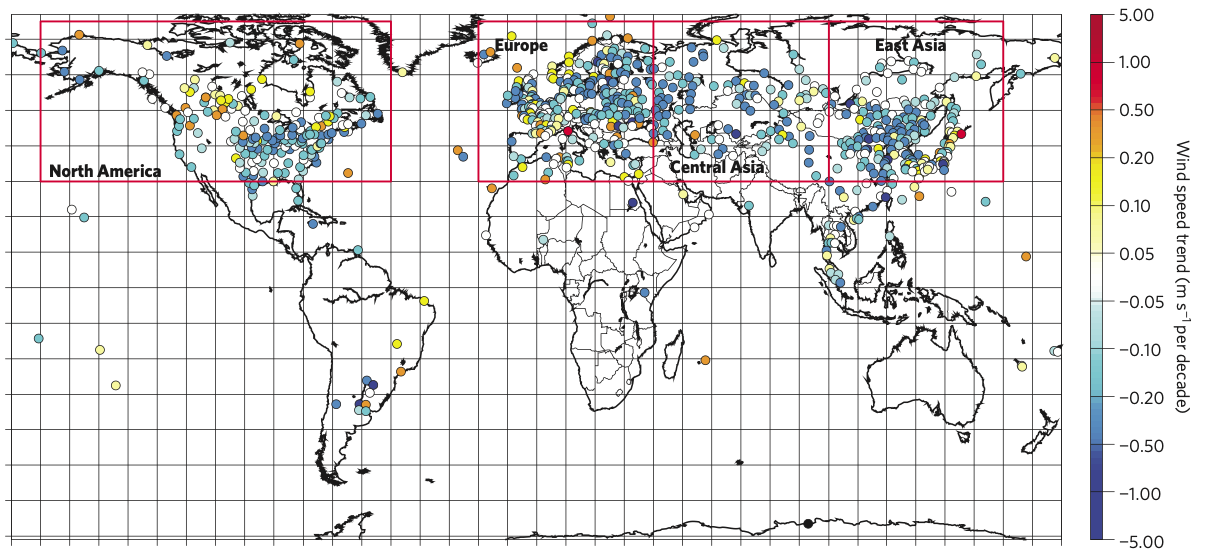
\includegraphics[width=1\textwidth]{北半球陆地地表风速趋势(Vautard等2010)}
    \bicaption{北半球陆地地表风速趋势。风速趋势使用1979-2008年地面观测计算得到。(来源:\citet{vautard2010northern})}{Land surface wind speed trends over the Northern Hemisphere. Wind speed trends were computed using surface observations from 1979 to 2016.(Source: \citet{vautard2010northern})}
    \label{fig:NHwindtrendVautard2010}
\end{figure}

\subsection{陆地地表风速长期变化的原因}

从动力学的角度,风速的变化满足下列关系:

\begin{equation} \label{eq:winddynmaic}
\frac{\mathrm{d} \vec{V}}{\mathrm{d} t} = \vec{G} + \vec{F} + \vec{g} + \vec{f}
\end{equation} ~\\
其中,$\vec{V}$为风矢量;$\vec{G} =\frac{1}{\rho} \nabla p $为气压梯度力,即为大气运动的驱动力,$\rho$ 为空气密度,$ p $为气压;$\vec{F} =-2 \Omega \times \vec{V} $为科里奥利力;$\vec{g}$ 为重力;$\vec{f}$为大气运动的阻力。由于科里奥利力和重力不会主动变化,因此,风速变化的可能原因可以分为两个方面:

\begin{enumerate}
 \item 大气运动驱动力的变化。大尺度的温度的变化会对大尺度大气运动驱动力产生影响,此外环流系统的变化也与大气运动驱动力变化密切联系。
 \item 大气运动阻力的变化。大气运动的阻力分为拖拽阻力和内部阻力,拖拽阻力主要由于城市化、植被变化等会引起地表粗糙度变化而产生;内部阻力主要则由于空气内部的湍流混合,与大气稳定度,风的垂直切变等有关。
\end{enumerate}

下面从主要从驱动力和阻力两个方面对前人研究进行回顾和总结:

\begin{enumerate}
\item 大气运动驱动力变化的影响

气温的不均匀变化可能会导致气压梯度力的变化,进而影响地表风速。\citet{klink1999trends}认为美国的地表风速变化可以由美国高纬度增温快于低纬度来解释。\citet{xu2006steady}认为冬季中国北部增温快于东边的西北太平洋,而夏季中国中部降温东边的西北太平洋增温,这使得东亚冬季风和夏季风均出现减弱,从而使得中国陆地地表风速减小。\citet{yan2002an}认为南半球变暖使得北大西洋风暴轴偏移,使得欧洲大陆风暴强度减小,从而使得欧洲陆地地表风速减小。

环流系统的变化会影响到地表风速。很多研究表明,北大西洋涛动(NAO)对欧洲陆地地表风速有显著影响\citep{beniston2005mountain, earl20131980–2010},而北极涛动(AO)与中国陆地地表风速有很好的相关\citep{chen2013wind}。此外,研究发现,厄尔尼诺南方涛动(ENSO)处于正为位相时,中国平均陆地地表风速相比ENSO负位相时高出$55 ~ \%$,表明ENSO对于中国陆地地表风速可能有影响\citep{chen2013wind}。\citet{wu2016estimating}发现,在东亚夏季风(EASM)强年,中国夏季陆地地表风速相比于EASM弱年高出$0.017 ~ m ~ s^{-1}$,表明了东亚夏季风可能影响中国陆地地表风速。近些年来,东亚季风有减弱的趋势\citep{zhu2012increases, ding2014interdecadal},也被认为是东亚陆地地表风速减小的原因之一\citep{xu2006steady}。

\begin{figure}[!htbp]
    \centering
    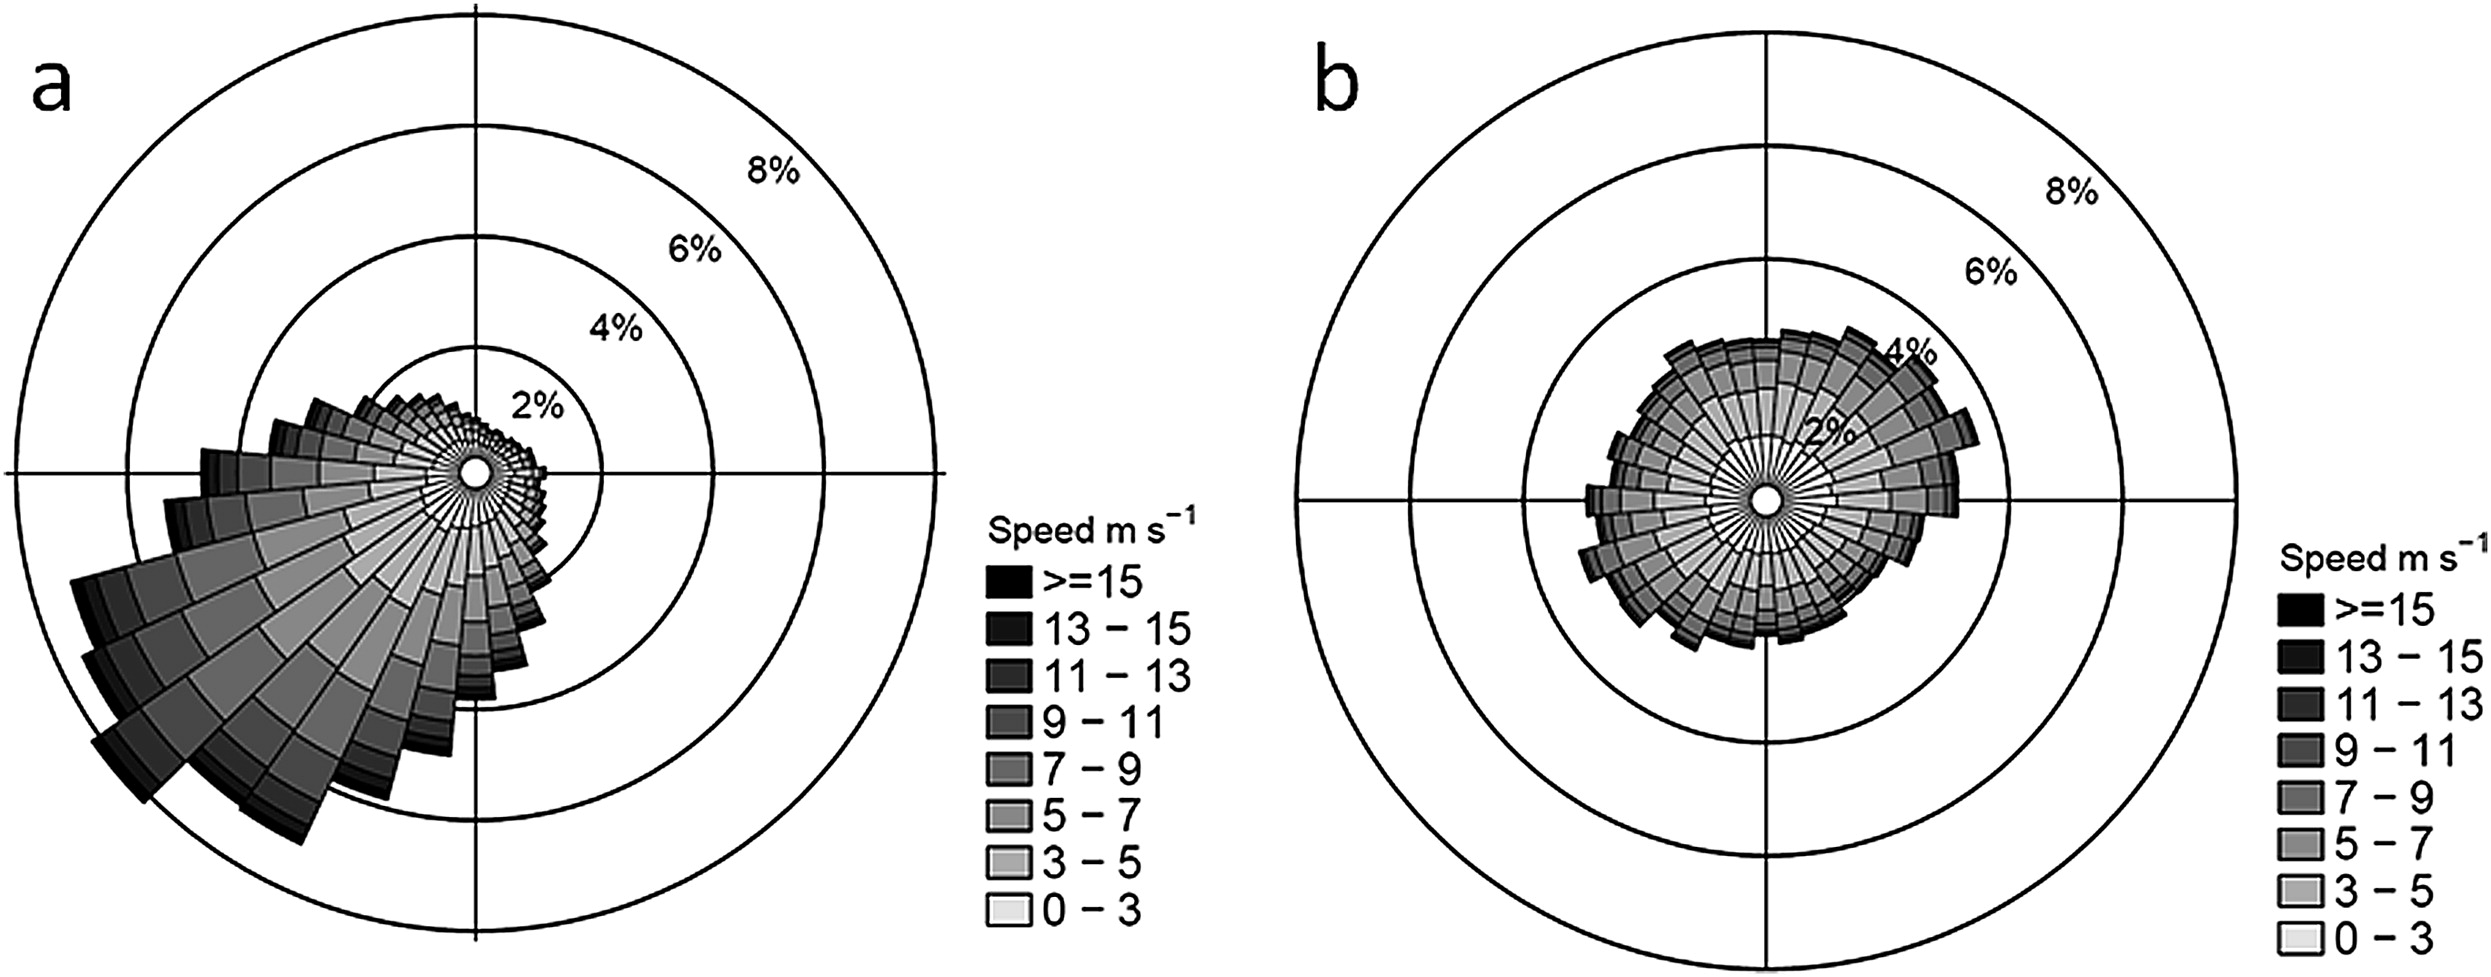
\includegraphics[width=1\textwidth]{英国地表风速与NAO(Earl等,2013)}
    \bicaption{不同NAO指数下的英国地表风。a)NAO指数大于2,b)NAO指数小于-2。(来源:\citet{earl20131980–2010})}{Surface winds over the United Kingdom under different NAO index. a)NAO index > 2, b)NAO index < -2. (Source: \citet{earl20131980–2010})}
    \label{fig:NAOUKwindEarl2013}
\end{figure}

\item 大气运动阻力变化的影响

如前文所述,观测陆地地表风速在近几十年来出现了显著减小,但海表风速却出现了增加\citep{tobin2014global, berrisford2015global, dunn2016surface},这从一定程度上反映了陆面拖拽阻力的变化对地表风速等影响。\citet{vautard2010northern}认为北半球陆地地表风速减弱的$25 – 60 ~ \%$可以由地表粗糙度变化解释。\citet{wever2012quantifying}发现欧洲地表粗糙度变化可以解释欧洲1981-2009年地表风速减弱的$70 ~ \%$。由于地表粗糙度观测数据的缺乏,地表粗糙度如何变化以及其对地表风速的影响难以直接考察,因而很多研究者采用了一些间接方式进行研究。例如,比较再分析资料(如NCEP/NCAR)与观测资料的差别来分析土地利用变化的影响\citep{kalnay2003impact, zha2017effects},比较城市与乡村站点风速变化来考察城市化的影响\citep{klaic2002modification, guo2011changes},也有利用数值试验来研究土地利用变化的影响\citep{vautard2010northern, zha2019numerical}。

\begin{figure}[!htbp]
    \centering
    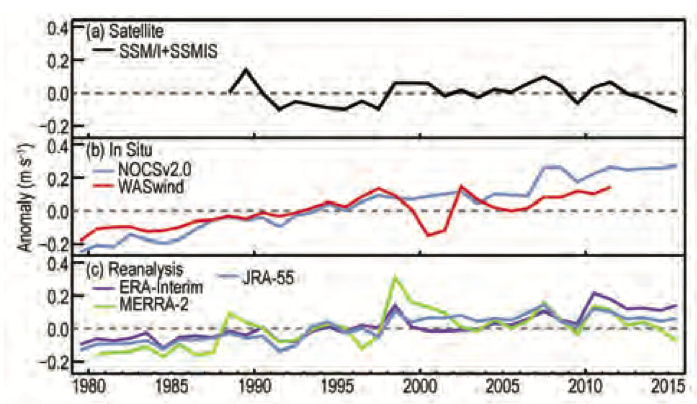
\includegraphics[width=0.9\textwidth]{海表风速变化(Dunn等,2016)}
    \bicaption{海表风速变化。a)卫星资料,b)观测资料,c)再分析资料。(来源:\citet{dunn2016surface})}{Changes in ocean surface winds. a) Satellite, b) In situ observation, c) Reanalysis. (Source: \citet{dunn2016surface})}
    \label{fig:Oceanwindchange}
\end{figure}

\begin{figure}[!htbp]
    \centering
    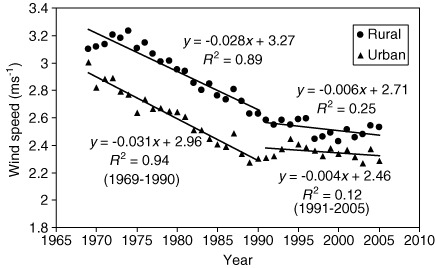
\includegraphics[width=0.95\textwidth]{中国城市化与风速变化(Guo等,2011)}
    \bicaption{中国城市与乡村风速变化,圆圈代表乡村站点风速,三角代表城市站点风速。(来源:\citet{guo2011changes})}{Wind speed evolution in urban and rural stations in China, circles denote rural station wind speeds, triangles denote urban station wind speeds . (Source: \citet{guo2011changes})}
    \label{fig:UrbanvsRuralChina}
\end{figure}

\begin{figure}[!htbp]
    \centering
    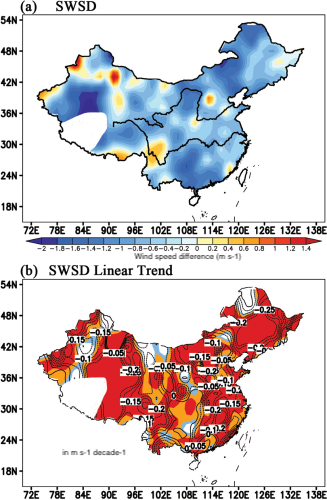
\includegraphics[width=0.85\textwidth]{中国地表风速OMR(Zha等,2017)}
    \bicaption{中国观测与再分析地表风速的差别。a)观测减ERA-Interim,b)观测减ERA-Interim的线性趋势。蓝色、黄色、红色区域分别代表显著性水平超过$90 ~ \%$、$95 ~ \%$和$99 ~ \%$(来源:\citet{zha2017effects})}{Observations minus reanalysis surface wind speeds over China. a) Observation minus ERA-Interim, b) Linear trends of observation minus ERA-Interim. Blue, yellow, and red area denote that the significance levels outreach $90 ~ \%$, $95 ~ \% $, and $99 ~ \%$, respectively. (Source: \citet{zha2017effects})}
    \label{fig:OMRchina}
\end{figure}


地表附近大气稳定度的变化会影响高层动量向下传递,从而影响地表风速。有研究表明,气溶胶和温室气体的变化可能改变大气稳定度\citep{ramanathan2005atmospheric, bichet2012causes}。气溶胶对于太阳辐射等吸收和反射会减少到达地面的短波辐射,从而增加大气稳定度。\citet{bichet2012causes}利用数值试验发现气溶胶增加使得印度和中国的地表风速分别减少了$ 0.13 ~ m ~ s^{-1}$和$0.03 ~ m ~ s^{-1}$。温室气体会使得不同层次的大气不均匀增温,从而改变大气的稳定度\citep{santer2011reproducibility}。\citet{bichet2012causes}的数值试验也探究了温室气体浓度对于地表风速的影响,但发现这种影响在1950年后并不显著。

\begin{figure}[!htbp]
    \centering
    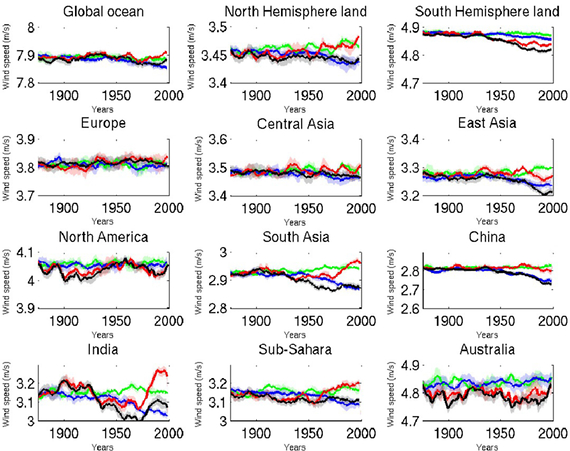
\includegraphics[width=1\textwidth]{外强迫对地表风速等影响(Bichet等,2012)}
    \bicaption{外强迫对地表风速等影响。黑线为控制试验,即包含所有外强迫,红线为气溶胶不变的情况,蓝线为海表温度保持不变的情况,绿色为气溶胶和海表温度均保持不变的情况(来源:\citet{bichet2012causes})}{Impact of external forcings on surface wind speed. Black line denotes control run, namely model run with all external forcings, red line denotes model run with aerosol remains unchanged, blue line denotes model run with sea surface temperature remains unchanged, and blue line denotes model run with aerosol and sea surface temperature remain unchanged. (Source: \citet{bichet2012causes})}
    \label{fig:ExternalForcing}
\end{figure}

\item 其他因素的影响

不可否认的是,一些人为因素同样会影响到观测的风速趋势,其中最主要的是观测仪器、规范以及观测环境的改变。\citet{mckee2000climate}指出,美国1990年左右安装的ASOS观测系统会使得大风风速相比之前的观测偏大,而小风风速偏小。\citet{刘学锋2012台站观测环境改变对我国近地面风速观测资料序列的影响}发现,台站障碍物视宽角对中国1971-2002年间地表风速趋势对贡献达到了1/3。

\end{enumerate}

\subsection{风能资源评估与变化}

\citet{archer2005evaluation}利用全球7753个地面观测站和446个探空观测站资料,计算了2000年全球的风能资源,发现风能资源总量相当于目前全球总用电量的约35倍,即约600PWh。\citet{lu2009global}利用模拟的风场资料计算了2006年全球未被林地、冰川覆盖,城市以外地区的风能资源,发现其总量超过当年全球总用电量的200倍,全球总能源消耗的25倍。一些工作评估了未来气候变化对于风能资源的可能影响,\citet{pryor2011assessing}利用CMIP5全球气候模式未来情景预估,使用区域气候模式降尺度之后发现,美国的近地面风能资源没有显著变化。\citet{karnauskas2018southward}发现,在未来预估情景下,北半球中纬度风能资源会减小,而热带地区和南半球风能资源会增加。

\begin{figure}[!htbp]
    \centering
    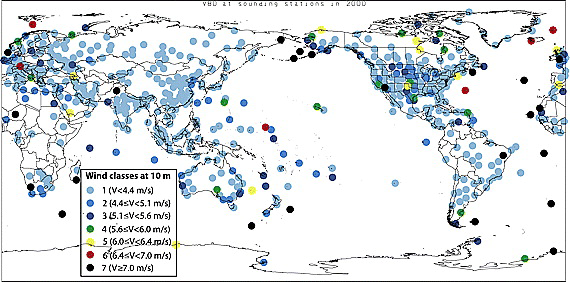
\includegraphics[width=1\textwidth]{风能资源分布(Archer和Jacobson,2005)}
    \bicaption{2000年风能资源分布。(来源:\citet{archer2005evaluation})}{Spatial distribution of wind energy resources in 2000. (Source: \citet{archer2005evaluation})}
    \label{fig:windenergyArcher2005}
\end{figure}

\section{论文主要内容}

从前面的回顾可以看出,陆地地表风速减弱是一个在全球普遍发生且颇为显著的现象,环流、温度、地表粗糙度等因素均可能对地表风速的变化产生影响。本文旨在于对大尺度陆地地表风速长期变化的相关问题做一个系统梳理,试图对以下问题作出回答:

\begin{enumerate}
\item 大尺度陆地地表风速的趋势,年代际变化有何特征?在不同区域,不同季节有何差别?
\item 大尺度陆地地表风速长期变化的背后的原因是什么?什么因素占主导作用?
\item 大尺度陆地地表风速长期变化对于风能资源有何影响?尤其对于风能资源较为丰富,有开发价值的地区的影响如何?
\end{enumerate}

由此,本文拟解决的主要科学问题如下:

\begin{enumerate}
\item 北半球陆地地表风速长期变化的时空特征

本文的分析主要以观测资料为基础,由于前期研究表明南半球高质量且长时间的地表风速序列较少,因而将主要研究区域选定为北半球。本文将北半球分为北美洲、欧洲、亚洲三个区域,对北半球总体状况和三个区域分别进行了分析,考察了陆地地表风速的长期趋势和年代际变化,以及在不同百分位,不同季节,不同高度的差别。由于仪器更换等人为误差的影响,观测地表风速长期变化存在不确定性,本文对比观测与多套再分析资料分析了这种不确定性。

\item 北半球陆地地表风速变化的机理

如前文所述,陆地地表风速变化的原因主要分为大气运动驱动力的变化和大气运动阻力的变化。本文从这两个方面出发,全面考察这两类变化的影响,包括海平面气压场、环流系统、大尺度海温、城市化、植被变化、大气稳定度等。

\item 北半球陆地地表风速长期变化对风能资源的影响

本文利用地面观测资料首先分析了北半球近38年来的风能资源整体状况,并筛选出了适于进行风能资源开发的地区,然后分析了陆地地表风速长期变化对风能资源的影响,特别是对于适于风能资源开发地区的影响。另外分析了全球气候模式对风能资源长期变化的模拟能力,以此作为评估全球气候模式风能资源预估可靠性的参考。

\end{enumerate}

论文章节安排如下:

第1章	\quad 绪论

第2章	\quad 北半球陆地地表风速长期变化的时空特征

第3章	\quad 大气运动驱动力变化对陆地地表风速长期变化的影响

第4章	\quad 大气运动阻力变化对陆地地表风速长期变化的影响

第5章	\quad 北半球陆地地表风速长期变化对风能资源的影响

第6章	\quad 总结与展望
